\selectlanguage{ngerman}%
\frenchspacing%
\begin{ledgroupsized}[r]{120mm}%
\footnotesize%
\pstart%
\noindent\textbf{Überlieferung:}%
\pend%
\end{ledgroupsized}%
\begin{ledgroupsized}[r]{114mm}%
\footnotesize%
\pstart%
\parindent -6mm%
\makebox[6mm][l]{\textit{L}}%
Aufzeichnung:
LH XXXVII~4, Bl.\;156.
Ein Zettel (16\;x\;13 cm);
Ränder beschnitten;
Papiererhaltungsmaßnahmen.
Eine halbe Seite jeweils auf Bl.\;156\,r\textsuperscript{o} und \;156\,v\textsuperscript{o};
Bl.\;156\,r\textsuperscript{o} überliefert zudem N.\;\ref{57037-3} %
sowie eine Notiz über Pyrotechnik %
und ein Fragment über die Gezeiten %
(beide sollen voraussichtlich in späteren Bänden von \textit{LSB} VIII ediert werden).
\pend%
\end{ledgroupsized}%
\selectlanguage{latin}%
\frenchspacing%
\vspace{5mm}%
\normalsize%
\pstart%
\noindent%
\lbrack%
\href{\Scan{LH_37_04_156r}}%
{156\,r\textsuperscript{o}}%
\rbrack%
\phantom{Augusti 1677}%
\hfill%
\phantom{\lbrack156\,r\textsuperscript{o}\rbrack}%
Augusti 1677
\pend%
\pstart%
\noindent%
\centering%
\edtext{%
Memorabile inventum%
\indexS{inventum memorabile}\\
Barometri%
\indexS{barometrum portabile}
et Thermometri%
\indexS{thermometrum portabile}
portatilis exactissimi%
}{%
\lemma{\textit{Am Rand%
:}}%
\Afootnote{%
$\displaystyle\frac{5}{4}$ Elle \mercury\ ohngefehr
pondus vel vis aeris.%
\indexS{pondus aeris}%
\indexS{vis aeris}
$\displaystyle\frac{1}{4}$ Elle \mercury\
est quinta virium portio.%
\indexS{portio virium}
Porro sit in spatio rarefacto%
\indexS{spatium rarefactum}
virium ut $\displaystyle\frac{5}{4}$
tantum vis ut $\displaystyle\frac{4}{4}$,
id est %
ejus quantitas sit ut 4 ad 5,
ad priorem.%
}}%
\pend%
\vspace{0.5em}%
\pstart%
\noindent%
\edtext{%
Sit Barometrum \textit{EABCD}%
\indexS{barometrum portabile}%
}{%
\lemma{Sit Barometrum \textit{EABCD}}%
\Cfootnote{%
Vgl. das Diagramm \lbrack\textit{Fig.\:1}\rbrack.%
}}
in quo Mercurius \textit{ABCD},%
\indexS{mercurius in barometro}
cujus altitudo \textit{AB}%
\indexS{altitudo mercurii}
eminet ultra horizontem \textit{BD}.%
\indexS{horizon}
Si \textit{EA} sit vacuum,%
\indexS{vacuum}
erit \textit{AB}
\edtext{%
altitudo Mercurii tantum%
\indexS{altitudo mercurii}
quantum sufficit ad aequipondium cylindri aerei.%
\indexS{aequipondium cylindri aerei}%
\indexS{cylinder aereus}%
}{%
\lemma{altitudo}%
\Bfootnote{%
\textit{(1)}~ad cyli %
\textit{(2)}~Mercurii tantum %
\lbrack...\rbrack\ aequipondium cylindri %
\textit{(a)}~aer %
\textit{(b)}~aerei.%
~\textit{L}%
}}
Sed si in \textit{EA} esset aliquod aeris,
minus tamen %
quam communiter esse solet,
foret Mercurius longe depressior%
\indexS{mercurius depressus}
seu minus altus,
\edtext{%
itaque aeris copiam%
}{%
\lemma{itaque}%
\Bfootnote{%
\textit{(1)}~aerem %
\textit{(2)}~aeris copiam%
~\textit{L}%
}}
pro arbitrio%
\indexS{arbitrium}
intus relinquendo,
possumus facere,
ut \textit{AB} Mercurius%
\indexS{mercurius in barometro}
ultra horizontem%
\indexS{horizon}
datae sit altitudinis.%
\indexS{altitudo mercurii}
Adjicimus autem Mercurio alium liquorem%
\indexS{liquor adjectus mercurio}
\edtext{%
\edlabel{LH_37_04_156-1_156r_hugenus-1}%
more%
\indexS{mos}
Hugenii%
\indexN{\textls{Huygens} (Hugenius, Ugenius, Hugens, Huguens), Christiaan 1629\textendash1695}%
\edlabel{LH_37_04_156-1_156r_hugenus-2}%
}{%
\lemma{more Hugenii}%
\Cfootnote{%
Siehe
\textsc{C.\;Huygens},
\glqq Extrait d'une autre lettre touchant une nouvelle maniere de Barometre\grqq\
(\textit{JS}, 12.~Dezember 1672, S.\;152--156;%
\cite{01522}
\textit{HO} VII, S.\;238--241).%
\cite{00113}%
}}
\edtext{%
et Cartesii.%
\indexN{\textls{Descartes} (Cartesius, des Cartes), René 1596\textendash1650}%
}{%
\lemma{et Cartesii}%
\Cfootnote{%
Siehe\cite{01471}
\textsc{P.\;Chanut}, %
Brief an F.\;Périer vom 24.\;September 1650 %
(in \textsc{B.\;Pascal}, \textit{Traitez}, Paris 1663, S.\;207\,f.;%
\cite{00081}
\textit{DO} V, S.\;476).%
\cite{00120}%
}}
Caeterum alia tunc instituenda erit
\edtext{%
divisio indicis.%
\indexS{divisio indicis}%
\indexS{index barometri}%
}{%
\lemma{divisio}%
\Bfootnote{%
\textit{(1)}~pro %
\textit{(2)}~indicis.%
~\textit{L}%
}}
Thermometro%
\indexS{thermometrum portabile}
res ita accomodari poterit,
uti
\edtext{%
\edlabel{LH_37_04_156-1_156r_hubinus-1}%
Hubinus%
\indexN{\textls{Hubin} (Hubinus), Louis (Ludion de) fl. 1673\textendash1683}
Barometrum Hugenii%
\indexN{\textls{Huygens} (Hugenius, Ugenius, Hugens, Huguens), Christiaan 1629\textendash1695}%
\indexS{barometrum Hugenii}
Thermometro accomodavit.%
\indexS{barometrum accomodatum thermometro}%
\indexS{thermometrum accomodatum barometro}%
\edlabel{LH_37_04_156-1_156r_hubinus-2}%
}{%
\lemma{Hubinus \lbrack...\rbrack\ accomodavit}%
\Cfootnote{%
Siehe
\textsc{L.\;Hubin},
\textit{Machines nouvellement executées}
(Paris 1673, S.\;10--12).\cite{01470}
Leibnizens Handexemplar ist in der GWLB Hannover unter der Signatur Leibn.\;Marg.\;129 aufbewahrt.%
}}
\pend%
\newpage%
\begin{edfigure}[0.0em][1.25em]
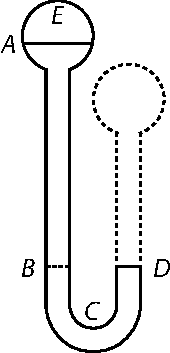
\includegraphics[width=0.16\textwidth]{gesamttex/edit_VIII-4/images/LH_37_04_156-1_d1_156r.pdf}
\edcaption[0.25em]
{\lbrack \textit{Fig.\:1}\rbrack%
\edtext{}{%
\lemma{\textit{Am Rand um das Diagramm} \lbrack\textit{Fig.\:1}\rbrack:}%
\Afootnote[nonum]{%
Nota%
\lbrack,\rbrack\
man kondte hier dabey haben die ponderatio\-nem%
\textsuperscript{\lbrack a\rbrack}
vacuae pilae%
\indexS{ponderatio pilae vacuae}%
\indexS{pila vacua}
so an dem liquore in die hohe ziehet.%
\indexS{liquor adjectus mercurio}
Item zu gleich Herrn Boyle%
\indexN{\textls{Boyle} (Boylius, Boyl), Robert 1627\textendash1691}
art nach die probe der Munzen,%
\indexS{Probe der Munzen}%
\indexS{Munze}%
\textsuperscript{\lbrack b\rbrack}
und ander dinge.
Durch das gewicht des schaffenleines%
\indexS{Schaffenlein}
würde man nachspüren
wiefiel es feuchtigkeit an sich gezogen:%
\indexS{Feuchtigkeit}
Nota %
melius mit einer gespanten chorde%
\indexS{chorda, gespant}
so sich drehet und einen Zeiger%
\indexS{Zeiger}
hat so sich mit drehet.%
\\[1ex]%
{\footnotesize%
\textsuperscript{\lbrack a\rbrack}~%
ponderationem
\textit{(1)}~der %
\textit{(2)}~vacuae pilae%
~\textit{L}%
\quad%
\textsuperscript{\lbrack b\rbrack}~%
Boyle \lbrack...\rbrack\ munzen:
Siehe
\textsc{R.\;Boyle},
\glqq A New Essay-Instrument\grqq\
(\textit{PT} X, 21.\;Juni 1675, S.\;329--348;\cite{01475}
\textit{BW}~VIII, S.\;532--544).\cite{00017}
Leibniz las möglicherweise aber die anonyme französische Zusammenfassung (\textit{JS}, 26.\;August 1675, S.\;223--225),
in der Boyles Messinstrument, anders als im englischen Original, explizit mit dem Barometer (\textit{aerometre}, S.\;223) verglichen wird.%
}%
}}%
}%
\end{edfigure}%
\pstart%
\noindent%
\lbrack%
\href{\Scan{LH_37_04_156v}}%
{156\,v\textsuperscript{o}}%
\rbrack\
Dieses Barometrum%
\indexS{barometrum portabile}
würde diesen Fehler haben,%
\indexS{Fehler barometri portabilis}
daß es zugleich ein
\edtext{%
\lbrack Therm\rbrack%
\indexS{thermometrum portabile}%
ome\-trum%
}{%
\lemma{Barometrum}%
\Bfootnote{%
\textit{L\;ändert Hrsg.}%
}}
were,
oder seine Indication%
\indexS{Indication}
aus beiden zusammengesezt.
Denn die in \textit{EA} sich befindende Lufft%
\indexS{Lufft, von der Wärme rarefaciert}
wurde von der Wärme%
\indexS{Wärme}
sich rarefaciren laßen%
\lbrack;\rbrack\
deßen ungeacht
wurden wir unsern Zweck erreichen,%
\indexS{Zweck}
\edtext{%
wann bey das Barometrum%
\indexS{barometrum portabile}%
}{%
\lemma{wann}%
\Bfootnote{%
\textit{(1)}~an dies Baro %
\textit{(2)}~bey das Barometrum%
~\textit{L}%
}}
ein Thermometrum%
\indexS{thermometrum portabile}
gefuget
\edtext{%
würde,
allein ich dencke an ein remedium%
\indexS{remedium}.%
}{%
\lemma{würde}%
\Bfootnote{%
\textit{(1)}~. Und dieses kondte meines bedünckens also %
\textit{(2)}~allein ich %
\lbrack...\rbrack\ ein remedium.%
~\textit{L}%
}}
\pend%
\pstart%
\edtext{%
Sit in \textit{EA} %
aer rarefactus%
\indexS{aer rarefactus}%
}{%
\lemma{Sit in \textit{EA}}%
\Cfootnote{%
Vgl. das Diagramm \lbrack\textit{Fig.\:2}\rbrack.%
}}%
\lbrack,\rbrack\
in
\edtext{%
\lbrack\textit{NM}\rbrack%
}{%
\lemma{\textit{LH}}%
\Bfootnote{%
\textit{L\;ändert Hrsg.}%
}}
adhuc rarefactior,
\textit{ABCD} barometrum%
\indexS{barometrum portabile}%
\indexS{barometrum apertum}
quod est apertum in \textit{D},
\edtext{%
et \textit{AGFHLMN}%
}{%
\lemma{et}%
\Bfootnote{%
\textit{(1)}~\textit{AF} %
\textit{(2)}~\textit{AGFHL} %
\textit{(3)}~\textit{AGFHLMN}%
~\textit{L}%
}}
thermometrum%
\indexS{thermometrum portabile}
\ledpb%
quod est clausum in \textit{N}.
Ope Mercurii \textit{AB}%
\indexS{mercurius in barometro}
\edtext{%
supra horizontem \textit{DBF} eminentis%
\indexS{horizon}%
}{%
\lemma{supra horizontem \textit{DBF} eminentis}%
\Bfootnote{%
\textit{erg.\;L}%
}}
erit aequilibrium%
\indexS{aequilibrium inter aerem externum et inclusum}
inter aerem externum ordinarium%
\indexS{aer externus}%
\indexS{aer ordinarius}
et aerem inclusum \textit{AE},%
\indexS{aer inclusus barometro}
rariorem externo.%
\indexS{aer rarior externo}
Et ope Mercurii \textit{LM}%
\indexS{mercurius in barometro}
supra horizontem \textit{AL}%
\indexS{horizon}
erit aequilibrium inter aerem rarum \textit{EA} %
et rariorem \textit{MN}.
\pend%
\pstart%
Verum
quia nihilominus calculo%
\indexS{calculus}
sive Tabula%
\indexS{tabula}
erit opus
et hoc
\edtext{%
modo duplo%
}{%
\lemma{modo}%
\Bfootnote{%
\textit{(1)}~nimis %
\textit{(2)}~duplo%
~\textit{L}%
}}
altius quam alias fiet instrumentum,%
\indexS{instrumentum}
necesse est
\textit{LM} esse satis altum%
\lbrack,\rbrack\
ideo satis erit sic agi:
sit thermometrum \textit{EAGFH}%
\indexS{thermometrum portabile}
et horizon \textit{DBF}%
\indexS{horizon}
\edtext{%
\lbrack et\rbrack%
}{%
\lemma{in}%
\Bfootnote{%
\textit{L\;ändert Hrsg.}%
}}
\textit{FH} pila plena aere%
\indexS{pila plena aere}
minus raro quam in \textit{EA},
et altitudo \textit{AF} Mercurii%
\indexS{altitudo mercurii}
aequilibrio serviet,%
\indexS{aequilibrium inter aerem externum et inclusum}
vel
\edtext{%
etiam quanta\lbrack m\rbrack\ volumus%
\lbrack;\rbrack\
in \textit{D}
et \textit{F}%
}{%
\lemma{etiam}%
\Bfootnote{%
\bars{quanta \textit{ändert Hrsg.}} volumus %
\textit{(1)}~, sive %
\textit{(2)}~in \textit{D} %
\textit{(a)}~, \textlangle siv\textrangle\ %
\textit{(b)}~, in \textit{F} %
\textit{(c)}~et \textit{F}%
~\textit{L}%
}}
superare poterunt liquores%
\indexS{liquor adjectus mercurio}
et habeatur
\edtext{%
Barometrum%
\indexS{barometrum portabile}
quale Hugenii,%
\indexN{\textls{Huygens} (Hugenius, Ugenius, Hugens, Huguens), Christiaan 1629\textendash1695}%
}{%
\lemma{Barometrum quale Hugenii}%
\Cfootnote{%
Siehe Erläuterung zu \refpassage{LH_37_04_156-1_156r_hugenus-1}{LH_37_04_156-1_156r_hugenus-2}.%
}}
et
\edtext{%
Thermometrum%
\indexS{thermometrum portabile}
quale Hubini%
\indexN{\textls{Hubin} (Hubinus), Louis (Ludion de) fl. 1673\textendash1683}%
}{%
\lemma{Thermometrum quale Hubini}%
\Cfootnote{%
Siehe Erläuterung zu \refpassage{LH_37_04_156-1_156r_hubinus-1}{LH_37_04_156-1_156r_hubinus-2}.%
}}
ad sensibilitatem.%
\indexS{sensibilitas barometri}%
\indexS{sensibilitas thermometri}
Everti poterit utcunque,
nec tamen quicquam effluet.
\pend%
\pstart%
Wenn am glas%
\indexS{Glas}
innewendig röllgen fest
kondte ein zeiger seyn,%
\indexS{Zeiger}
oder wiederumb vis mechanica.%
\indexS{vis mechanica}
\pend%
\begin{edfigure}[0.5em][0.0em]
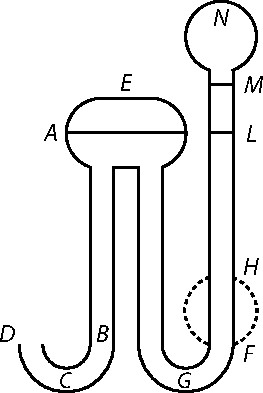
\includegraphics[width=0.28\textwidth]{gesamttex/edit_VIII-4/images/LH_37_04_156-1_d2_156v.pdf}
\edcaption%
{%
\lbrack \textit{Fig.\:2}\rbrack%
\edtext{}{%
\lemma{\textit{Um das Diagramm} \lbrack\textit{Fig.\:2}\rbrack:}%
\Afootnote[nonum]{%
Opus Tabula quadrata
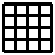
\includegraphics[width=0.03\textwidth]{gesamttex/edit_VIII-4/images/LH_37_04_156-1_d3_156v.pdf}
drauff zu schreiben die combinationes.%
}}%
}%
\end{edfigure}%
\selectlanguage{latin}%
\frenchspacing%
\normalsize%
